

We build up a coarse-grained molecular dynamics model to simulate the NPC systems with LAMMPS, get the trajectory of each production run, then analyze the result using VMD.

\subsection*{The Coarse-Grained Model}
\begin{figure}[h!]
\begin{center}
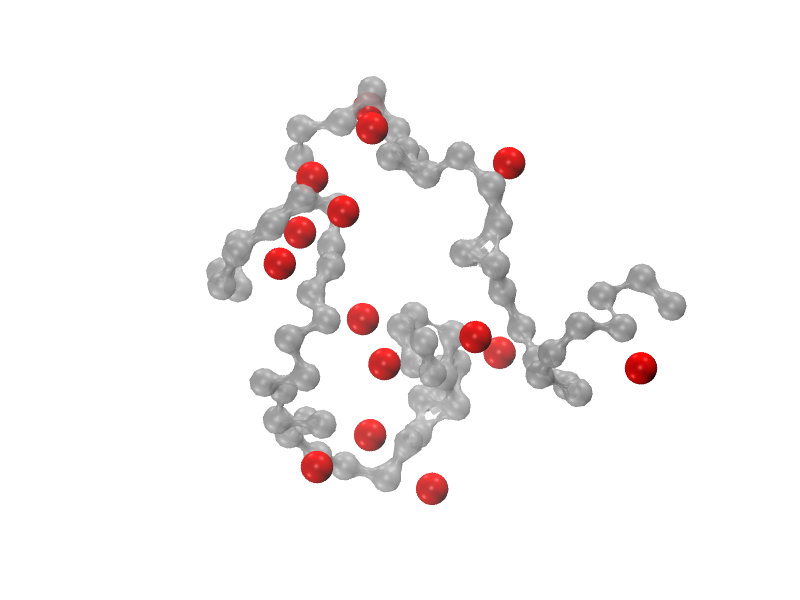
\includegraphics[width=5in]{./figure/pnp.png}
\caption{A snapshot of the CG PNC system, taken with VMD.~\cite{Humphrey1996a}}
\label{fig:pnp_snapshot}
\end{center}
\end{figure}
Using Self-Avoid Walking (SAW) method, we firstly put $N$ polymer chains into a cubic Periodic Boundary Condition (PBC) box. There are $L$ monomers in each chain, and the mass of each monomer is $56$ representing a sum of $4$ carbon and $8$ hydrogen atoms. All bond lengths are set to $4.7~\AA$. Then we put $M$ fillers into the system randomly.~\ref{fig:pnp_snapshot}

The force field we use in our model is simply the Lennard-Jones potential (L-J potential) {eq.~\ref{eq:lj}}, we modify it according to our desire to the L-J potential with radii cut at some certain distance (eq.~\ref{eq:lj_cut}).

\begin{equation}\label{eq:lj}
p^{LJ}(r_{i,j})=4\epsilon_{i,j}\left[ \left(\frac{\sigma_{i,j}}{r_{i,j}}\right)^{12}-\left(\frac{\sigma_{i,j}}{r_{i,j}}\right)^6 \right]
\end{equation}

\begin{equation}\label{eq:lj_cut}
p(r_{i,j})=
\left\{
\begin{array} {l l}
p^{LJ}(r_{i,j}) - p^{LJ}(r_{c}) & \quad (r_{i,j}<r_{c}) \\
0 & \quad (r_{i,j} \geq r_{c})
\end{array} 
\right.
\end{equation}

$\epsilon_{i,j}$ and $\sigma_{i,j}$ are respectively the strength of the interaction, and the equilibration distance of the interacting atom-pair $i, j$ under consideration.

\subsection*{Protocols of Molecular Dynamics Simulation}
After all chains and fillers are positioned in our PBC box, the PNC system is minimized using ${NVE}$ with a limitation imposed on the distance that atoms are allowed to move in one timestep, in our system, $0.05\AA/fs^{-1}$. When the energy of the system reaches the minimum, we compress the system and equilibrate it at $1000K$ (which is adjustable), and then lower it stepwise by the decrement of $50K$, to our desired temperture $T_{eq}$ (i.e., $200K$ in our compression simulation, and $600K$ in the shearing one), the whole procedure is performed using ${NVT}$ updates by far. Equilibrated under $T_{eq}$, the system is then relaxed using ${NPT}$ updates to the pressure $P_{eq}$. The system is ready for any molecular dynamics production run.

\subsubsection*{The Tensiling}
$1.1\times10^{-5}\AA/fs$

\subsubsection*{The Compression}
During the compression procedure, we use the so-called $NL_x\sigma_y\sigma_z T$ ensemble, under which we compress the system along the $X$-axis, and keep the pressure on other directions unchanged at $T_{eq}$. The rate of the compression is $1.0\times10^{-11}\AA/fs$.

\subsubsection*{The Shearing}

\subsection*{Setup of the Systems}
Here is the list of the potential parameters in each system (the substripts $p$ and $f$ represents polymer and filler respectively, the energy unit is $KCal/mol$ and the length unit is $\AA$):
\begin{table}[h!]
\begin{center}
\vspace*{0.5cm}
\begin{threeparttable}
\begin{tabular}{lcccccc}
\hline
Simulation & System & $\epsilon_{p,p}$ & $\sigma_{p,p}$ & $\epsilon_{p,f}$\tnote{*} & $\sigma_{p,f}$\tnote{\dag}\\
\hline
S1 & Polymer     & $1.13$         & $4.7$ &    -    & -     \\
S2 & Polymer-LF  & $1.13$         & $4.7$ & $4.52$  & $9.2$ \\
S3 & Polymer-MF  & $1.13$\tnote{*}& $4.7$ & $4.52$  & $6.1$ \\
S4 & Polymer-SF  & $1.13$         & $4.7$ & $4.52$  & $4.6$ \\
\hline
\end{tabular}
\begin{tablenotes}
\item[*] \small{we keep $\sigma_{f,f}=0.25\sigma_{p,p}$ for all systems.}
\item[\dag] \small{Except $r_{cp,f}=2.1\sigma$, $r_{c}=2.1\sigma$ for all $i,j$ atom-pairs}
\end{tablenotes}
\end{threeparttable}
\caption{List of simulations}
\label{simu_summary}
\end{center}
\end{table}
\iffalse
我们初步建立了四类体系,各体系里包含128条含有64个粗粒化单元的高分子链和不同的纳米颗粒(表1)。
表 1 体系参数
2. 力场
	我们将Dilip Gersappe研究PNC拉伸屈服机理[6]提出的模型进行了改进,参数则采用了Aki Kutvone 等人研究复合材料拉伸[8]时的设置。
高分子键 如公式1,在高分子链上两个相邻成键的粗粒化单元间,采用2-4谐振子势。本模型中没有设置高分子链的键角及二面角作用势。
    ,                   (1)
非键作用势 体系内非键连的粒子间都为LJ作用势,如公式2所示。对于高分子粗粒化单元间相互作用,σ=σext,ε=εext 。对于纳米颗粒间的相互作用,εnp=0.25εext ,σ的值为各体系中纳米颗粒的直径σL、σM、σS 。对于纳米颗粒与高分子单元间的相互作用,εpnp=4εext ,σ=(σext+σnp)/2。同一高分子链内的两个非键粗粒化单元间相互作用,截断半径为2^(1/6)σ,其余非键作用的粗粒化粒子截断半径均为2.1σ。具体参数见表2。
 ,                                 (2)
表 2  力场参数
kh	rh0	εext	σext	σS	σM	σL
11.62	4.7	1.13	4.7	4.6	6.1	9.2
注:上图中能量单位为kcal,长度单位为Å

3.模拟过程
	\fi